\documentclass{article}
\usepackage[margin=1in]{geometry}
\usepackage{tikz}
\usepackage{pgfplots}

\pgfplotsset{compat=1.18}

\begin{document}

% ---------- Shared legend ----------
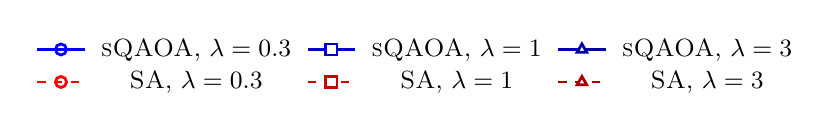
\begin{tikzpicture}
\begin{axis}[
    hide axis,
    xmin=0, xmax=1,
    ymin=0, ymax=1,
    legend columns=3,
    legend style={draw=none, fill=none, font=\small, column sep=0.35em}
]
\addlegendimage{blue, mark=o, mark options={solid, fill=white}, line width=1pt}
\addlegendentry{\textsc{sQAOA}, $\lambda=0.3$}
\addlegendimage{blue!80!black, mark=square*, mark options={solid, fill=white}, line width=1pt}
\addlegendentry{\textsc{sQAOA}, $\lambda=1$}
\addlegendimage{blue!65!black, mark=triangle*, mark options={solid, fill=white}, line width=1pt}
\addlegendentry{\textsc{sQAOA}, $\lambda=3$}
\addlegendimage{red, dashed, mark=o, mark options={solid, fill=white}, line width=1pt}
\addlegendentry{\textsc{SA}, $\lambda=0.3$}
\addlegendimage{red!80!black, dashed, mark=square*, mark options={solid, fill=white}, line width=1pt}
\addlegendentry{\textsc{SA}, $\lambda=1$}
\addlegendimage{red!65!black, dashed, mark=triangle*, mark options={solid, fill=white}, line width=1pt}
\addlegendentry{\textsc{SA}, $\lambda=3$}
\end{axis}
\end{tikzpicture}

\begin{figure}[t]
\centering
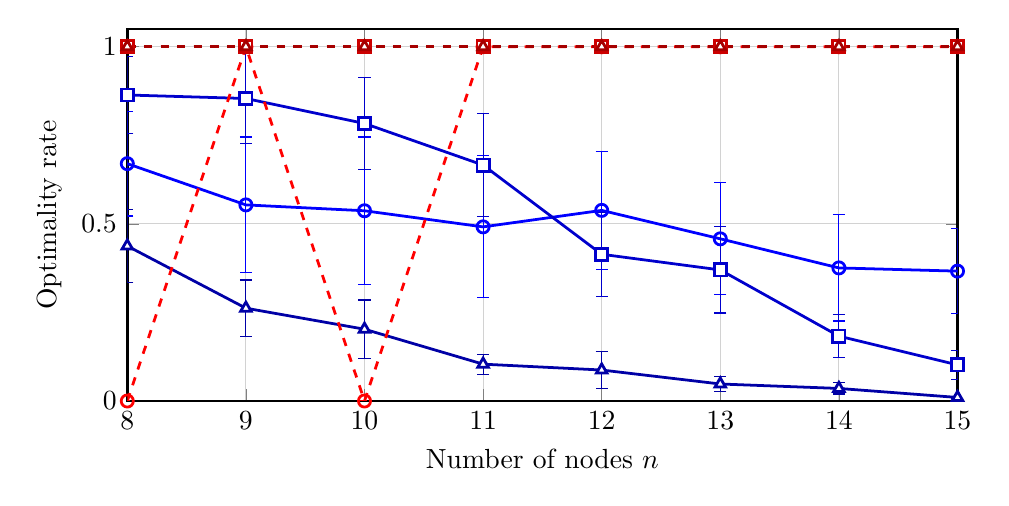
\begin{tikzpicture}
\begin{axis}[
    width=\linewidth,
    height=0.52\linewidth,
    xlabel={Number of nodes $n$},
    ylabel={Optimality rate},
    xmin=8, xmax=15,
    ymin=0, ymax=1.05,
    xtick={8,9,10,11,12,13,14,15},
    grid=both,
    grid style={gray!20},
    major grid style={gray!35},
    line width=1pt,
    mark size=2.2pt,
]

\addplot+[blue, mark=o, mark options={solid, fill=white}, error bars/.cd, y dir=both, y explicit] coordinates {
    (8,0.670000) +- (0,0.147596)
    (9,0.553602) +- (0,0.191733)
    (10,0.537037) +- (0,0.208364)
    (11,0.491573) +- (0,0.200516)
    (12,0.538121) +- (0,0.165671)
    (13,0.457814) +- (0,0.158182)
    (14,0.375685) +- (0,0.149790)
    (15,0.366608) +- (0,0.119754)
};
\addplot+[blue!80!black, mark=square*, mark options={solid, fill=white}, error bars/.cd, y dir=both, y explicit] coordinates {
    (8,0.863869) +- (0,0.107969)
    (9,0.853980) +- (0,0.126126)
    (10,0.783441) +- (0,0.130669)
    (11,0.666000) +- (0,0.145481)
    (12,0.414209) +- (0,0.118821)
    (13,0.370000) +- (0,0.121655)
    (14,0.183161) +- (0,0.060193)
    (15,0.102000) +- (0,0.041415)
};
\addplot+[blue!65!black, mark=triangle*, mark options={solid, fill=white}, error bars/.cd, y dir=both, y explicit] coordinates {
    (8,0.437557) +- (0,0.102900)
    (9,0.262000) +- (0,0.079468)
    (10,0.202649) +- (0,0.082534)
    (11,0.104000) +- (0,0.028085)
    (12,0.087444) +- (0,0.052396)
    (13,0.048000) +- (0,0.020080)
    (14,0.035448) +- (0,0.015771)
    (15,0.010000) +- (0,0.002829)
};
\addplot+[red, dashed, mark=o, mark options={solid, fill=white}, error bars/.cd, y dir=both, y explicit] coordinates {
    (8,0.000000) +- (0,0.000000)
    (9,1.000000) +- (0,0.000000)
    (10,0.000000) +- (0,0.000000)
    (11,1.000000) +- (0,0.000000)
    (12,1.000000) +- (0,0.000000)
    (13,1.000000) +- (0,0.000000)
    (14,1.000000) +- (0,0.000000)
    (15,1.000000) +- (0,0.000000)
};
\addplot+[red!80!black, dashed, mark=square*, mark options={solid, fill=white}, error bars/.cd, y dir=both, y explicit] coordinates {
    (8,1.000000) +- (0,0.000000)
    (9,1.000000) +- (0,0.000000)
    (10,1.000000) +- (0,0.000000)
    (11,1.000000) +- (0,0.000000)
    (12,1.000000) +- (0,0.000000)
    (13,1.000000) +- (0,0.000000)
    (14,1.000000) +- (0,0.000000)
    (15,1.000000) +- (0,0.000000)
};
\addplot+[red!65!black, dashed, mark=triangle*, mark options={solid, fill=white}, error bars/.cd, y dir=both, y explicit] coordinates {
    (8,1.000000) +- (0,0.000000)
    (9,1.000000) +- (0,0.000000)
    (10,1.000000) +- (0,0.000000)
    (11,1.000000) +- (0,0.000000)
    (12,1.000000) +- (0,0.000000)
    (13,1.000000) +- (0,0.000000)
    (14,1.000000) +- (0,0.000000)
    (15,1.000000) +- (0,0.000000)
};

\end{axis}
\end{tikzpicture}
\caption{Optimality rate with error bars showing standard error across five runs.}
\label{fig:r3-d5-100-optimality}
\end{figure}

\begin{figure}[t]
\centering
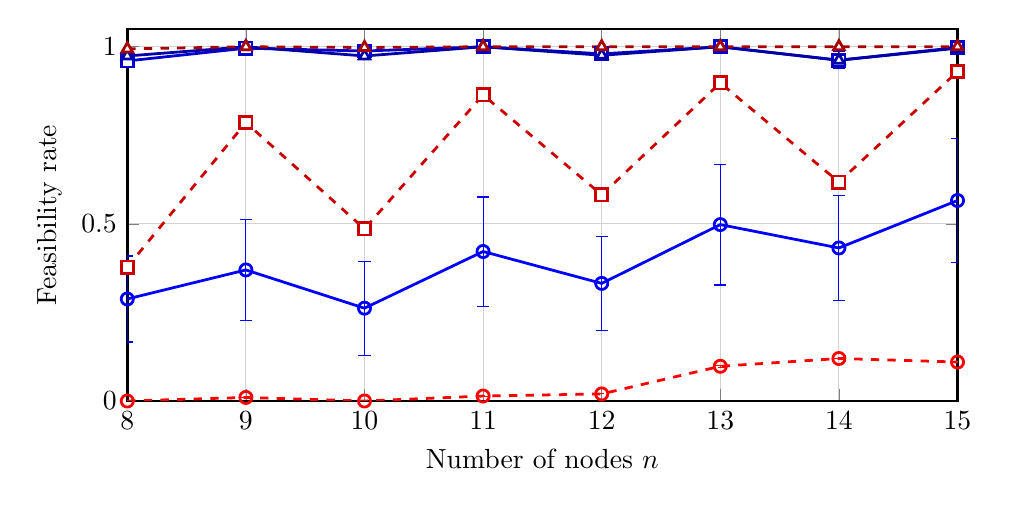
\begin{tikzpicture}
\begin{axis}[
    width=\linewidth,
    height=0.52\linewidth,
    xlabel={Number of nodes $n$},
    ylabel={Feasibility rate},
    xmin=8, xmax=15,
    ymin=0, ymax=1.05,
    xtick={8,9,10,11,12,13,14,15},
    grid=both,
    grid style={gray!20},
    major grid style={gray!35},
    line width=1pt,
    mark size=2.2pt,
]

\addplot+[blue, mark=o, mark options={solid, fill=white}, error bars/.cd, y dir=both, y explicit] coordinates {
    (8,0.288000) +- (0,0.121372)
    (9,0.370000) +- (0,0.142070)
    (10,0.262000) +- (0,0.132406)
    (11,0.422000) +- (0,0.154023)
    (12,0.332000) +- (0,0.131800)
    (13,0.498000) +- (0,0.170585)
    (14,0.432000) +- (0,0.148146)
    (15,0.566000) +- (0,0.174736)
};
\addplot+[blue!80!black, mark=square*, mark options={solid, fill=white}, error bars/.cd, y dir=both, y explicit] coordinates {
    (8,0.960000) +- (0,0.009381)
    (9,0.996000) +- (0,0.002191)
    (10,0.988000) +- (0,0.004382)
    (11,1.000000) +- (0,0.000000)
    (12,0.980000) +- (0,0.011314)
    (13,1.000000) +- (0,0.000000)
    (14,0.962000) +- (0,0.023732)
    (15,0.998000) +- (0,0.001789)
};
\addplot+[blue!65!black, mark=triangle*, mark options={solid, fill=white}, error bars/.cd, y dir=both, y explicit] coordinates {
    (8,0.974000) +- (0,0.008764)
    (9,1.000000) +- (0,0.000000)
    (10,0.974000) +- (0,0.009633)
    (11,1.000000) +- (0,0.000000)
    (12,0.976000) +- (0,0.008294)
    (13,1.000000) +- (0,0.000000)
    (14,0.962000) +- (0,0.011454)
    (15,0.996000) +- (0,0.003578)
};
\addplot+[red, dashed, mark=o, mark options={solid, fill=white}, error bars/.cd, y dir=both, y explicit] coordinates {
    (8,0.000000) +- (0,0.000000)
    (9,0.010000) +- (0,0.000000)
    (10,0.000000) +- (0,0.000000)
    (11,0.014000) +- (0,0.002191)
    (12,0.020000) +- (0,0.000000)
    (13,0.098000) +- (0,0.003346)
    (14,0.120000) +- (0,0.000000)
    (15,0.110000) +- (0,0.000000)
};
\addplot+[red!80!black, dashed, mark=square*, mark options={solid, fill=white}, error bars/.cd, y dir=both, y explicit] coordinates {
    (8,0.378000) +- (0,0.008672)
    (9,0.786000) +- (0,0.010040)
    (10,0.486000) +- (0,0.007798)
    (11,0.864000) +- (0,0.014311)
    (12,0.582000) +- (0,0.015849)
    (13,0.898000) +- (0,0.013682)
    (14,0.618000) +- (0,0.011099)
    (15,0.930000) +- (0,0.006324)
};
\addplot+[red!65!black, dashed, mark=triangle*, mark options={solid, fill=white}, error bars/.cd, y dir=both, y explicit] coordinates {
    (8,0.994000) +- (0,0.003578)
    (9,1.000000) +- (0,0.000000)
    (10,0.998000) +- (0,0.001789)
    (11,1.000000) +- (0,0.000000)
    (12,1.000000) +- (0,0.000000)
    (13,1.000000) +- (0,0.000000)
    (14,1.000000) +- (0,0.000000)
    (15,1.000000) +- (0,0.000000)
};

\end{axis}
\end{tikzpicture}
\caption{Feasibility rate with error bars showing standard error across five runs.}
\label{fig:r3-d5-100-feasibility}
\end{figure}

\end{document}
